\section{カメラキャリブレーション}
\label{calib}

はじめにカメラの内部パラメータ(焦点距離,歪み係数)を計算するためにカメラキャリブレーションを行う\cite{calib}.
ここで得られるパラメータはカメラ毎に固有の値となる為新しいカメラを利用する場合は毎回行う必要がある.

今回はOpenCVのfindChessboardCorners関数\cite{cvcalib}を用いてチェスボード\ref{chessboard}の格子点を検出し,
そのデータを用いてcalibrateCamera関数を用いてキャリブレーションを行った\ref{calib_code}.
キャリブレーションには一マス2.40cmの正方形が縦8マス横11マスに並ぶチェスボードと呼ばれる格子模様の画像100枚を利用してキャリブレーションを行った.

\begin{lstlisting}[caption=calibration code,label=calib_code]
def calib(self, frame):                                                                                                                                      
    image = cv2.cvtColor(frame, cv2.COLOR_RGB2BGR)                                                                                                           
    square_size = 2.4                                                                                                                                        
    pattern_size = (7, 10)                                                                                                                                   
    reference_img = 100                                                                                                                                      
                                                                                                                                                            
    pattern_points = np.zeros((np.prod(pattern_size), 3), np.float32)                                                                                        
    pattern_points[:, :2] = np.indices(pattern_size).T.reshape(-1, 2)                                                                                        
    pattern_points *= square_size                                                                                                                            
                                                                                                                                                            
    if len(self.objpoints) < reference_img:                                                                                                                  
        gray = cv2.cvtColor(image, cv2.COLOR_BGR2GRAY)                                                                                                       
                                                                                                                                                            
        ret, corner = cv2.findChessboardCorners(gray, pattern_size)                                                                                          
        print(corner)                                                                                                                                        
        if ret is True:                                                                                                                                      
            print(str(len(self.objpoints)+1) + "/" + str(reference_img))                                                                                     
            term = (cv2.TERM_CRITERIA_EPS + cv2.TERM_CRITERIA_COUNT, 30, 0.1)                                                                                
            cv2.cornerSubPix(gray, corner, (5, 5), (-1, -1), term)                                                                                           
            self.imgpoints.append(corner.reshape(-1, 2))                                                                                                     
            self.objpoints.append(pattern_points)                                                                                                            
                                                                                                                                                            
        cv2.imshow('image', image)                                                                                                                           
        if cv2.waitKey(200) & 0xFF == ord('q'):                                                                                                              
            pass                                                                                                                                             
    else:                                                                                                                                                    
        gray = cv2.cvtColor(image, cv2.COLOR_BGR2GRAY)                                                                                                       
        print("calculating camera parameter...")                                                                                                             
        ret, mtx, dist, rvecs, tvecs = cv2.calibrateCamera(                                                                                                  
            self.objpoints, self.imgpoints, gray.shape[::-1], None, None)                                                                                    
                                                                                                                                                            
        np.save("tello_mtx", mtx)                                                                                                                            
        np.save("tello_dist", dist.ravel())                                                                                                                  
        print("RMS = ", ret)                                                                                                                                 
        print("mtx = \n", mtx)                                                                                                                               
        print("dist = ", dist.ravel())                                                                                                                       
\end{lstlisting}

\begin{figure}[htbp]
  \begin{center}
    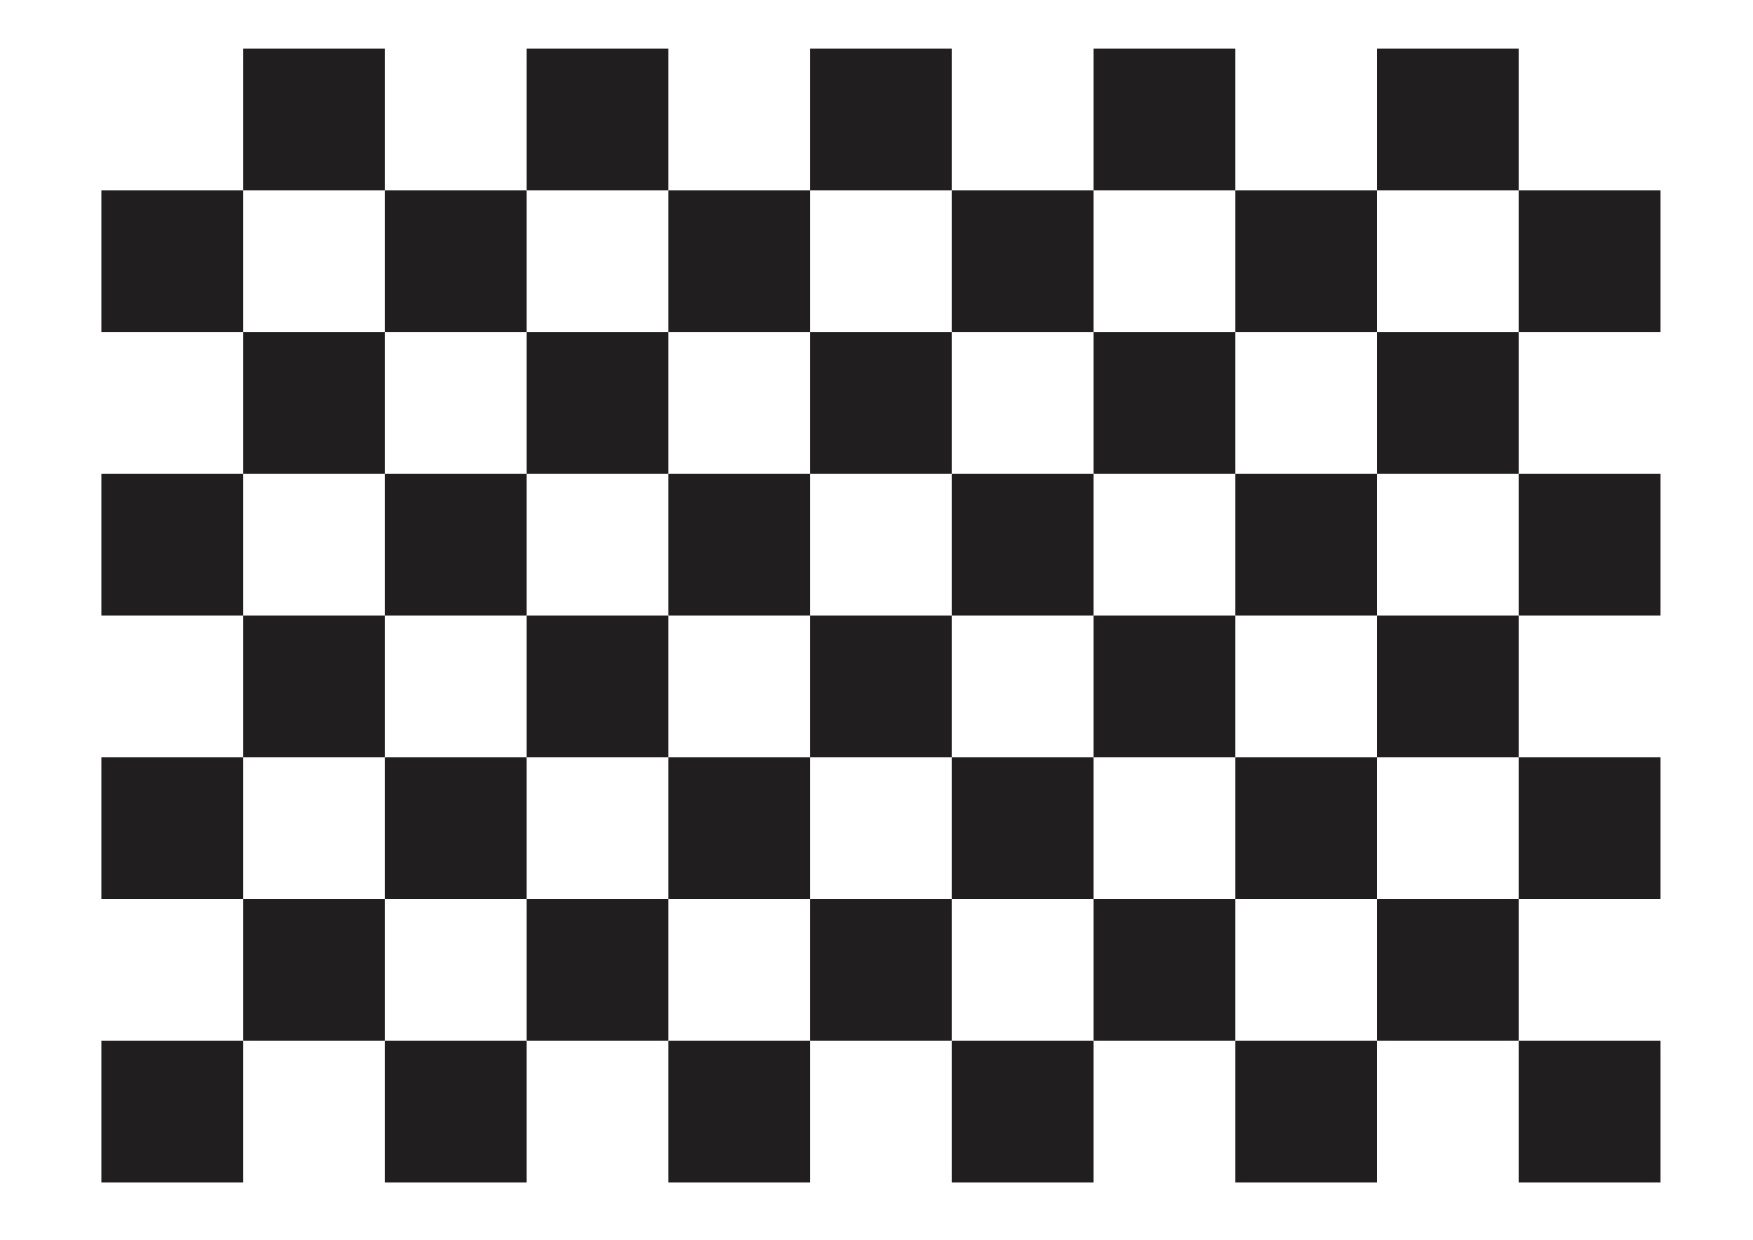
\includegraphics[clip,width=15.0cm]{img/chessboard.jpg}
    \caption{縦8マス横11マスのチェスボード}
    \label{chessboard}
  \end{center}
\end{figure}